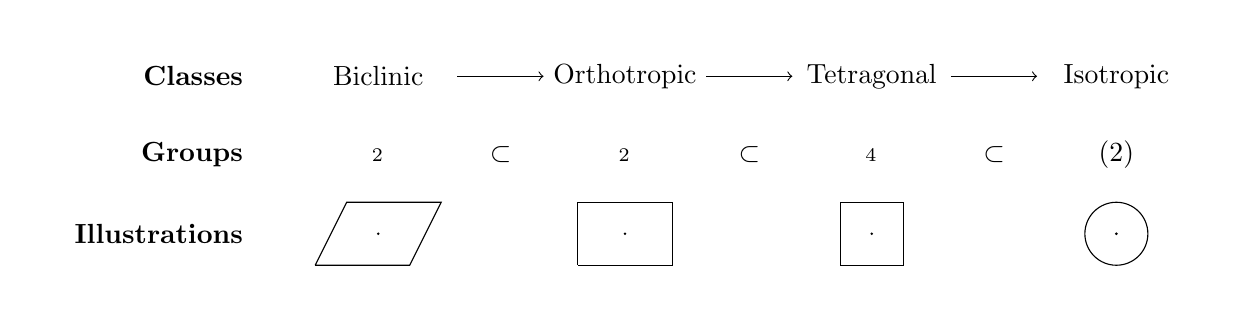
\begin{tikzpicture}[
        header/.style={align=right, minimum height=1cm, text width=2.5cm},
        cell/.style={align=center, minimum height=2em, minimum width=2cm},
    ]
    % Create a matrix
    \matrix [column sep=0.3cm] {
        % Symmetry classes
        \node[header] {\textbf{Classes}};  &
        &
        \node[cell] (bic) {Biclinic};               &
                                                    &
        \node[cell] (ort) {Orthotropic};            &
                                                    &
        \node[cell] (cub) {Tetragonal};             &
                                                    &
        \node[cell] (iso) {Isotropic};              \\
        % Groups
        \node[header] {\textbf{Groups}};            &
        &
        \node[cell] (zz2) {$\ZZ_2$};                &
        \node {$\subset$};                          &
        \node[cell] (dd2) {$\DD_2$};                &
        \node {$\subset$};                          &
        \node[cell] (dd4) {$\DD_4$};                &
        \node {$\subset$};                          &
        \node[cell] (oo2) {$\OO(2)$};               \\
        % Geometric figures
        \node[header] {\textbf{Illustrations}}; &
        &
        \fill[black] (0,0) circle (0.5pt); \draw (-0.6-0.2,-0.4) -- (-0.6+0.2,0.4) -- (0.6+0.2,0.4) -- (0.6-0.2,-0.4) -- (-0.6-0.2,-0.4);  &
        &
        \fill[black] (0,0) circle (0.5pt); \draw (-0.6,-0.4) -- (-0.6,0.4) -- (0.6,0.4) -- (0.6,-0.4) -- (-0.6,-0.4);  &
        &
        \fill[black] (0,0) circle (0.5pt); \draw (-0.4,-0.4) -- (-0.4,0.4) -- (0.4,0.4) -- (0.4,-0.4) -- (-0.4,-0.4);  &
        &
        \fill[black] (0,0) circle (0.5pt); \draw (0,0) circle (0.4);                                                 \\
    };
    % Add paths
    \draw[->] (bic) -- (ort);
    \draw[->] (ort) -- (cub);
    \draw[->] (cub) -- (iso);
\end{tikzpicture}
